\chapter{Results and Discussion}
\label{chapterlabel3}

\section{Preliminary \Beas-\Bmag\ Comparison: Results} \label{prelim results}
The angle between \Beas\ and \Bmag\ vectors, when plotted alongside those vectors for randomly chosen sample data from 31st August 2023, yields Figure \ref{fig: angle example august}.
\\

\begin{figure}[h!]
    \centering
    \centerfloat
    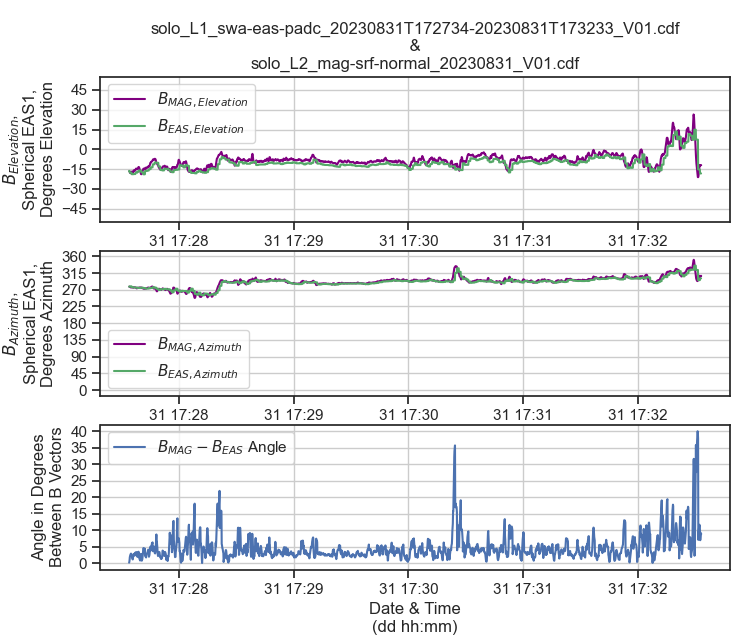
\includegraphics[width=1.05\linewidth]{figures/Angle Example.png}
    \caption{Example \(B_{EAS}\) data from a 5 minute period of EAS Burst Mode on 31st August 2023. Top panel: Elevation for \(B_{EAS}\) and \(B_{MAG}\) in spherical EAS1. Middle panel: Azimuth for \(B_{EAS}\) and \(B_{MAG}\) in spherical EAS1. Bottom panel: Angular difference between \(B_{EAS}\) and \(B_{MAG}\).}
    \caption*{Image Source: Author's own work}
    \label{fig: angle example august}
\end{figure}

\begin{figure}[h!]
    \centering
    \centerfloat
    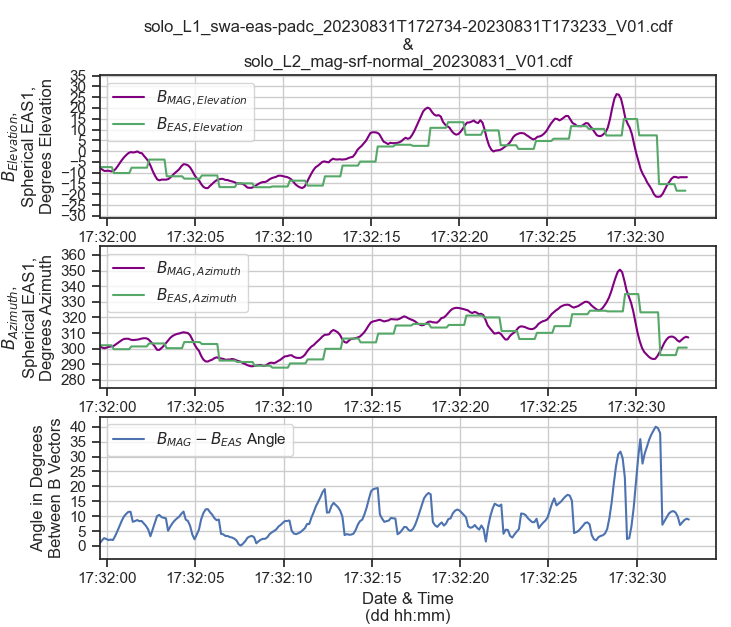
\includegraphics[width=1.05\linewidth]{figures/Angle Example Detail.png}
    \caption{A detailed look at the last \(\sim5\)s of Figure \ref{fig: angle example august}. Top panel: Elevation for \(B_{EAS}\) and \(B_{MAG}\) in spherical EAS1. Middle panel: Azimuth for \(B_{EAS}\) and \(B_{MAG}\) in spherical EAS1. Bottom panel: Angular difference between \(B_{EAS}\) and \(B_{MAG}\).}
    \caption*{Image Source: Author's own work}
    \label{fig: angle example detail august}
\end{figure}

By inspection, while relatively good agreement can be seen between \(B_{EAS}\) and \(B_{MAG}\) over long timescales, there are clear discrepancies over short timescales as shown in Figure \ref{fig: angle example detail august}. An unexpected observation is that \(B_{EAS}\) has less time resolution than \(B_{MAG}\), appearing only to update at 1Hz. Inspection of the raw \q{SWA\_EAS\_MagDataUsed} data time series data reveals that while this data array \textit{is} published to SOAR with 8 vectors for every second of \q{EPOCH} as advertised, these vectors are only updated once per second, resulting in 8 identical vectors per second such that the effective cadence is 1Hz. Since these data are packaged in L1 \textit{.cdf} files, they are expected to represent the true MAG data used to steer EAS, which implies that the alleged 1/8th second resolution of EAS Burst Mode is compromised by a magnetic field vector only updates at 1Hz. This will be a particular source of error during periods of fast-changing magnetic field. This effective 1Hz effect has been observed in other periods of Burst Mode from the sample including 5th November 2023 and 1st January 2023. It is absent from the relatively quiet period on 30th May 2023. Further research is required to determine the cause for this unexpectedly low update cadence, and how widespread of an issue this is in the SOAR dataset.
\\

The highest angular offset in Figure \ref{fig: angle example august} is observed to exceed 40\(\degree\), and it exceeds 70\(\degree\) in a different example from 5th November 2023. Otherwise, the offset is between \(0\degree\) and \(10\degree\) for \(\sim82\%\) of the period in Figure \ref{fig: angle example august}. In comparison, the offset varies between \(3\degree\) and \(5\degree\) for \(\sim80\%\) of the period in a different example from 30th May 2023, and between \(6\degree\) and \(8\degree\) for the remaining period. The bin centers and bin widths for elevation and azimuth are tabulated with level 2 EAS data files. While azimuth bins are identical for both heads, elevation bins are different due to minor differences in the assembly of each EAS head's electron optics. These tables have been updated over time but remained constant from 17th July 2021 until January 2024, when they were reverted to a previous version due to the error described in Section \ref{sim steering}. The tables from that 2021-2024 period are discussed here and are included in Appendix \ref{appendixlabel1}. The widest angular bin in EAS1 has width \(\pm6.06\degree\). This is well below much of the angular offset observed in the sample, therefore, it is established that \Beas\ could be sufficiently offset from \Bmag\ to cause erroneous Burst Mode steering, justifying the development of a metric for PAD quality/completeness.
\newpage

\section{SWA-DPU Binning Algorithm} \label{sim steering}

\begin{figure}[h!]
    \centering
    \centerfloat
    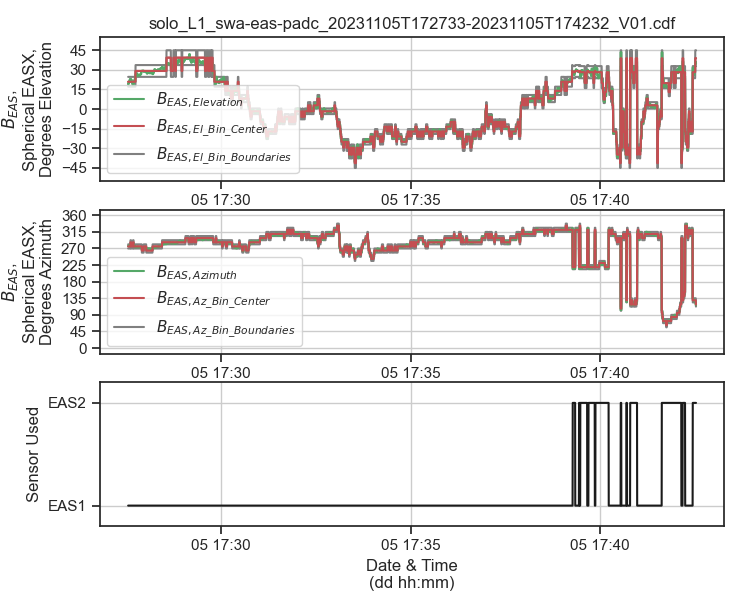
\includegraphics[width=1.05\linewidth]{figures/Steering Example.png}
    \caption{Example \(B_{EAS}\) data from a 15-minute period of EAS Burst Mode on 5th November 2023 showing a simulation of the Burst Mode steering algorithm. The reference frame for the top two panels is labelled \q{EASX} to indicate that it switches between EAS1 and EAS2 over the 15 minute period depending on \(B_{EAS}\) orientation and resulting head selection. Top panel: Elevation for \(B_{EAS}\) in spherical EASX coordinates, along with the centers and upper/lower bounds of the selected elevation bins (\q{El\_Bin\_Center} and \q{El\_Bin\_Boundaries} respectively). Middle panel: Azimuth for \(B_{EAS}\) in spherical EASX coordinates, along with the centers and upper/lower bounds of the selected azimuth bins (\q{Az\_Bin\_Center} and \q{Az\_Bin\_Boundaries} respectively). Bottom panel: The selected head over time.}
    \caption*{Image Source: Author's own work}
    \label{fig: steering example november}
\end{figure}

In the interest of validating the simulated binning algorithm described in Section \ref{sim steering - method}, the simulated binning for parallel \Beas\ vectors is plotted in Figures \ref{fig: steering example november} and \ref{fig: steering example november detail} along with a plot of the chosen head over time, for a 15-minute period on 5th November 2023. Figure \ref{fig: steering example november} shows that the elevation and azimuth values \q{jump} as the reference frame switches from EAS1 to EAS2 towards the end of the time series. As expected, this switch can be triggered by the \(B_{EAS}\) elevation exceeding \(\pm45\degree\) in its previous head's reference frame. Figure \ref{fig: steering example november detail} provides a detailed view of the algorithm's selection of appropriate binning such that the \(B_{EAS}\) trace stays between bin boundaries.
\\

\begin{figure}[h!]
    \centering
    \centerfloat
    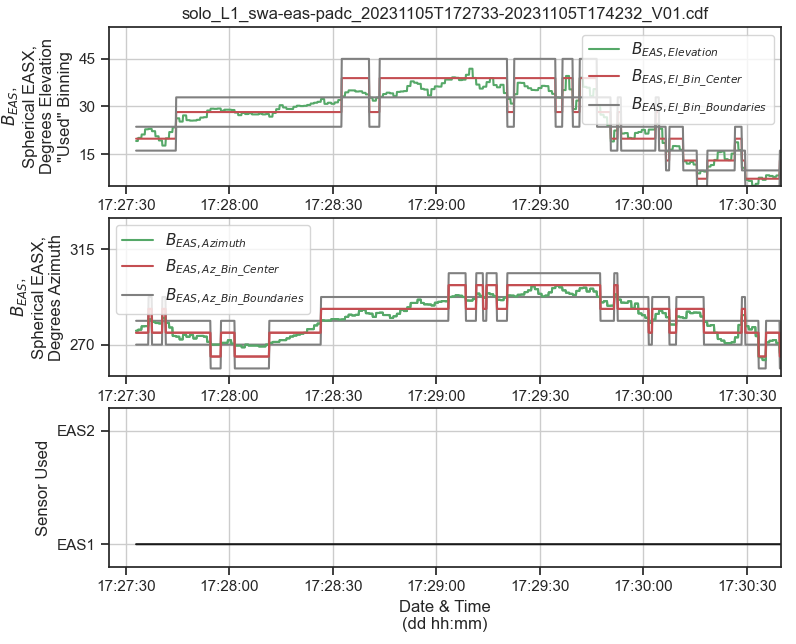
\includegraphics[width=1.05\linewidth]{figures/Steering Example Detail Start.png}
    \caption{A detailed view of the first \(\sim2.5\) minutes of Figure \ref{fig: steering example november}. Top panel: Elevation + binning for \(B_{EAS}\) in spherical EASX coordinates. Middle panel: Azimuth + binning for \(B_{EAS}\) in spherical EASX coordinates. Bottom panel: The selected head over time.}
    \caption*{Image Source: Author's own work}
    \label{fig: steering example november detail}
\end{figure}

In the interest of validating the binning algorithm even further, a more direct comparison was performed using the \q{Used} bin data directly from SOAR \textit{.cdf} files. Plotting the \q{Used} heads and elevation bins in an attempt to recreate Figure \ref{fig: steering example november} yields Figure \ref{fig: november bin error}. While the \q{SWA\_EAS\_EasUsed} head is perfectly correlated with the calculated head in the bottom panel of Figure \ref{fig: november bin error}, the top panel shows that not only does the \q{SWA\_EAS\_ELEVATION} binning appear to disagree with the simulated binning in the top panel of Figure \ref{fig: november bin error}, but the \q{Used} binning also appears to capture the \Beas\ elevation inaccurately over long periods of the time series. This is shown more clearly in Figure \ref{fig: november bin error detail}. In an attempt to fix this discrepancy, the data binning code was reviewed and multiple variations of the elevation bin tables were applied to the simulated algorithm. A possible bug was considered that might have caused the bin tables for the two heads to be swapped, but swapping them manually did not fix the discrepancy. The possibility that the uploaded data on SOAR had been reverted to a previous version was also considered, and older bin tables available on SOAR from 19th August 2020 to 17th July 2021, and from Solar Orbiter's commissioning to 19th August 2020 were also applied, but these did not fix the discrepancy either. The discrepancy was brought to the attention of the Principal Investigator of Solar Orbiter SWA (Dr. Chris Owen) and the SWA operations team, and Solar Orbiter was commanded to downlink the binning tables in its memory along with routine housekeeping data. The data downlink revealed that Solar Orbiter had, indeed, been using outdated bin tables in the SWA-DPU onboard, explaining the failure of \q{SWA\_EAS\_ELEVATION\_delta\_lower} and \q{SWA\_EAS\_ELEVATION\_delta\_upper} to encapsulate \Beas. 
\\

\begin{figure}[h!]
    \centering
    \centerfloat
    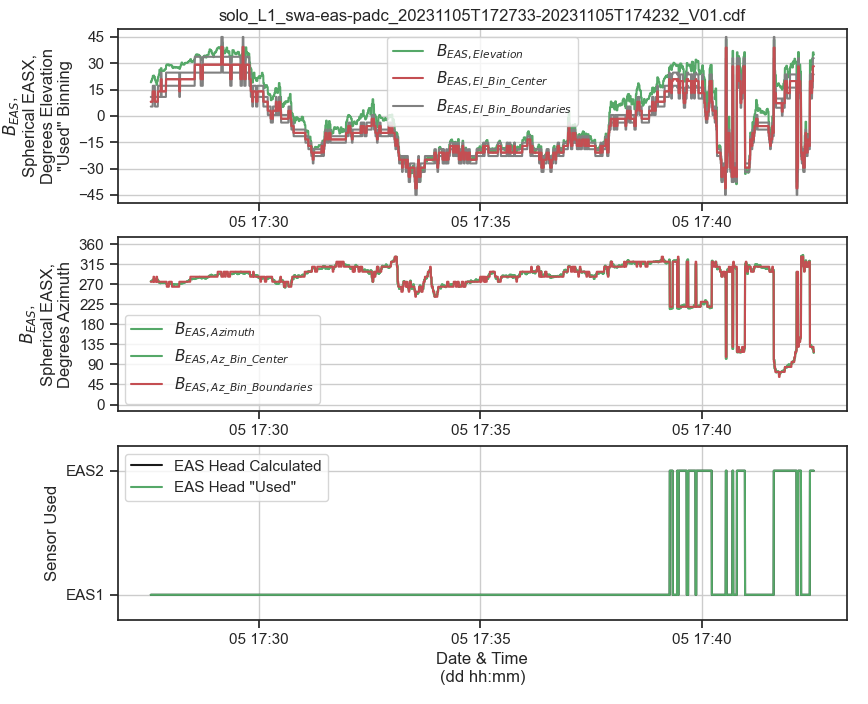
\includegraphics[width=1.05\linewidth]{figures/Steering Example (bin issue).png}
    \caption{Similar data to Figure \ref{fig: steering example november}, but plotting the \q{Used} bin centers, bin bounds, and sensor heads. Top panel: Elevation for \(B_{EAS}\) in spherical EASX coordinates, along with centers and upper/lower bounds of the used elevation bins (\q{El\_Bin\_Center} and \q{El\_Bin\_Boundaries} respectively). Middle panel: Azimuth for \(B_{EAS}\) in spherical EASX coordinates, along with the centers and upper/lower bounds of selected azimuth bins (\q{Az\_Bin\_Center} and \q{Az\_Bin\_Boundaries} respectively). Bottom panel: The selected, or \q{Calculated} head and used head over time.}
    \caption*{Image Source: Author's own work}
    \label{fig: november bin error}
\end{figure}

\begin{figure}[h!]
    \centering
    \centerfloat
    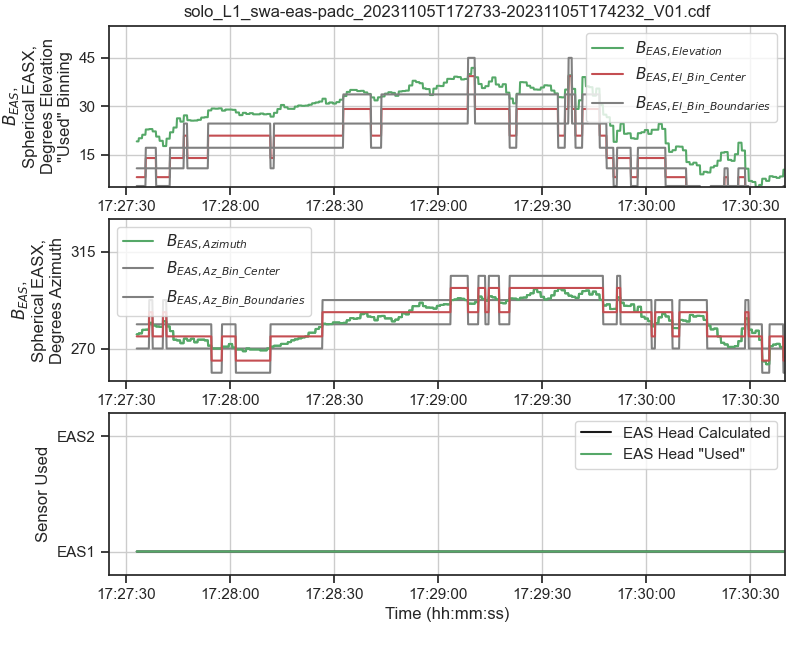
\includegraphics[width=1.05\linewidth]{figures/Steering Example Detail Start (bin issue).png}
    \caption{A detailed view of the first \(\sim2.5\) minutes of Figure \ref{fig: steering example november}. Top panel: Elevation + used binning for \(B_{EAS}\) in spherical EASX. Middle panel: Azimuth + binning for \(B_{EAS}\) in spherical EASX. Bottom panel: The selected, or \q{Calculated} head and used head over time.}
    \caption*{Image Source: Author's own work}
    \label{fig: november bin error detail}
\end{figure}

A partial explanation for this issue is that the SWA-DPU uses one bin table to steer the EAS heads to a particular elevation, and a different bin table to separate electron counts into elevation bins for further processing. While the second table may have been correctly updated, the first (\q{steering}) table had either not been updated or had been unintentionally reverted to an earlier state. Only the binning for the second table is uploaded to SOAR under \q{SWA\_EAS\_ELEVATION}. The effect that this mismatch can have on elevation binning is illustrated by Figure \ref{fig: bin issue cartoon}, where the vertical position of each yellow circle represents the elevation value associated with an individual electron. In Burst Mode, the elevation of the received \Bmag\ vector is first binned according to the steering table (Figure \ref{fig: bin issue cartoon}, left). When EAS is then steered to the appropriate elevation bin (e.g. \q{bin 0}), that bin is \q{filled} with electron detections from various elevations within its elevation boundaries, represented by the bins filled with yellow circles in Figure \ref{fig: bin issue cartoon}, left. In order to label these raw electron detection data with their appropriate elevation angles, SWA-DPU then uses the indices of the \q{filled} bins (0-15) in the \textit{other} binning table in Figure \ref{fig: bin issue cartoon}, right. While there is some overlap between bins with the same indices in both tables, the tables are mostly mismatched. Therefore, while some electron detections are correctly represented by both tables, this can lead the labelled elevation data to incorrectly report that certain elevation ranges are less \q{filled} with electron detections than reality. This is represented by the bins that are partially filled with electron detections in Figure \ref{fig: bin issue cartoon}, right. 
\\

This is the explanation for bin table mismatch which was found only to affect EAS Burst Mode data (which involves steering and therefore a steering table) prior to 2024. However, because of this project, it was later discovered that both the steering table \textit{and} the table uploaded to SOAR had been incorrect since 1st January 2024, compromising both Burst Mode and Normal Mode data. As a result, as of 22nd July 2024, all EAS data since 1st January 2024 have been expunged from SOAR\cite{soar}.

\begin{figure}[h!]
    \centering
    \centerfloat
    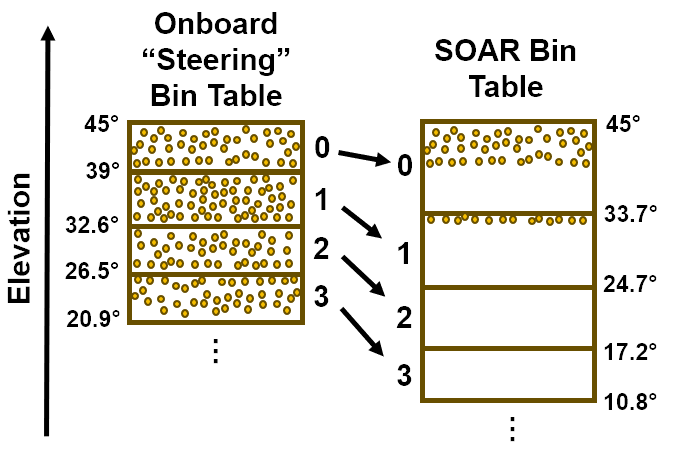
\includegraphics[width=0.75\linewidth]{figures/bin issue cartoon.png}
    \caption{A cartoon to illustrate the process by which a discrepancy in the two elevation binning tables used by SWA DPU can lead to incorrect elevation binning. The vertical axis indicates the elevation angle corresponding to various electron detections, which are represented by yellow circles. The first four bins for the two binning tables are represented by rectangles labelled with their indices and the angles of their upper and lower elevation bounds, and vertically scaled according to their elevation widths. The short arrows indicate the correspondence between the indices of the mismatched binning tables.}
    \caption*{Image Source: Author's own work}
    \label{fig: bin issue cartoon}
\end{figure}

\newpage
\section{Completeness Algorithm} \label{completeness}
Research into the steering algorithm and data visualisation completed earlier in this project made it clear that there is a relatively fast approach to generating a \q{completeness} or \q{quality} score for Burst Mode PADs, circumventing the relatively expensive process of re-binning EAS Burst Mode VDF data to generate the PADs in the first place, and then assessing PAD completeness \q{by hand} (e.g. by counting the white bins in Figure \ref{fig: PAD example}).
\\

As previously described, while discrepancies between \(B_{EAS}\) and \(B_{MAG}\) are expected to cause some inaccuracies in Burst Mode PADs, the resulting PADs will only be left \textit{incomplete} if these discrepancies disrupt Burst Mode steering. That is, under otherwise-ideal conditions, in order to lose part of a \([0\degree-180\degree)\) distribution, not only must \(B_{EAS}\) lie within a different angular bin than \(B_{MAG}\), but, more specifically, it must lie within a different \textit{elevation} bin than the actual bin(s) selected. Differences in azimuthal bin selection would lead the pitch angles recovered from the azimuthal bins in each selected elevation band (e.g. as shown in Figure \ref{fig: normal - full contours + selection}) to be labelled incorrectly, but this can be corrected in post-processing as long as \(B_{MAG}\) is known. No amount of re-labelling can recover a pitch angle that would have fallen within an elevation bin that was not sampled. The exact amount of pitch angle \q{loss} therefore only depends on the elevation angles of \(B_{MAG}\) and the selected elevation bins. Consider the vector parallel to \(B_{EAS}\), whose selected elevation bin is meant to capture a range of pitch angles from 0\degree\ (for the pixel containing the vector) to \(\geq90\degree\) (for the pixel in the same elevation bin with \(+180\degree\) azimuth compared to the vector). If \(B_{MAG}\) lies outside of this elevation bin, then, after re-labelling pitch angle data, the smallest pitch angle that can be recovered is theoretically equal to the smallest difference in elevation between \(B_{MAG}\) and each of the two boundaries (upper and lower) of the selected parallel elevation bin. Any electron with a pitch angle smaller than this difference is travelling too close to parallel with \(B_{MAG}\) to be captured by the selected elevation bin and therefore goes undetected. More formally, let \(B_{EAS, \ppara}\), \(B_{EAS, \apara}\), \(B_{MAG, \ppara}\), and \(B_{MAG, \apara}\) represent the unit vectors parallel and anti-parallel to \(B_{EAS}\) and \(B_{MAG}\) respectively. Working in the selected EAS head frame, the pitch angle loss \(\Delta_{\ppara}\) associated with \(B_{EAS, \ppara}\) is given by:

\begin{equation} \label{eq: parallel loss}
    \Delta_{\ppara}=\min\{|\theta_{MAG, \ppara}-\theta_{upper, \ppara}|, |\theta_{MAG, \ppara}-\theta_{lower, \ppara}|\}
\end{equation}

where \(\theta_{MAG, \ppara}\) is the elevation of \(B_{MAG, \ppara}\) and \(\theta_{upper, \ppara}\) and \(\theta_{lower, \ppara}\) are the elevations of the upper and lower boundaries of the selected parallel elevation bin respectively. \(\Delta_{\ppara}\) is equivalent to the minimum theoretical pitch angle \(\alpha_{min}\) that can be recovered from a Burst Mode PAD, yielding the identity:

\begin{equation} \label{eq: alpha min}
    \alpha_{min}=\Delta_{\ppara}
\end{equation}

Similarly, the pitch angle loss \(\Delta_{\apara}\) associated with \(B_{EAS, \apara}\) is given by:

\begin{equation} \label{eq: antiparallel loss}
    \Delta_{\apara}=\min\{|\theta_{MAG, \apara}-\theta_{upper, \apara}|, |\theta_{MAG, \apara}-\theta_{lower, \apara}|\}
\end{equation}

where \(\theta_{MAG, \apara}\) is the elevation of \(B_{MAG, \apara}\) and \(\theta_{upper, \apara}\) and \(\theta_{lower, \apara}\) are the elevations of the upper and lower boundaries of the selected anti-parallel elevation bin respectively. As before, \(\Delta_{\apara}\) implies that any electrons with a pitch angle larger than a maximum theoretical pitch angle \(\alpha_{max}\) cannot be detected. Therefore, if all angles are expressed in degrees, then the maximum theoretical pitch angle that can be recovered from a Burst Mode PAD is given by:

\begin{equation} \label{eq: alpha max}
    \alpha_{max}=180\degree-\Delta_{\apara}
\end{equation}

Notably, the fact that pitch angle loss occurs first at an \(\alpha_{min}\) and \(\alpha_{max}\) at either end of a full PAD before \q{spreading} towards the center of the distribution may imply that EAS Burst Mode is particularly ineffective at capturing narrow electron strahl populations in the solar wind, which are aligned with \(B_{MAG, \ppara}\) or \(B_{MAG, \apara}\) by definition\cite{kajdic2016}.
\\

In general, it should \textit{not} be assumed that \(\Delta_{\ppara}=\Delta_{\apara}\) because the specific elevation bins associated with \(B_{EAS, \ppara}\) and \(B_{EAS, \apara}\) are calculated independently of each other and, in general, the elevation bins for both sensor heads are of non-uniform width\cite{owen2020}\cite{owen2021}. In other words, a loss of \(\Delta_{\ppara}\) with respect to the parallel bin does \textit{not} imply a symmetric and equal loss \(\Delta_{\apara}\) with respect to the anti-parallel bin. This asymmetry can be captured using the visualisation tool described in Section \ref{visualisation}. Using pre-existing code for plotting pitch angle contours, \(\alpha_{min}\) and \(\alpha_{max}\) can be treated as any other pitch angle and visualised in the same way as the pitch angles in Figures \ref{fig: normal - full contours} and Figure \ref{fig: normal - full contours + selection}. When \(\alpha_{min}\) and \(\alpha_{max}\) are visualised this way, the sizes (or \q{radii}) of their contours around \(B_{MAG, \ppara}\) and \(B_{MAG, \apara}\) on the plot represent the sizes of the losses \(\Delta_{\ppara}\) and \(\Delta_{\apara}\) respectively.  Using the period of Burst Mode data from 12th June 2023 as an example, \(\alpha_{min}\) and \(\alpha_{max}\) are presented in Figure \ref{fig: full contours + selection + loss} as pitch angle contours plotted in red around \(B_{EAS, \ppara}\) (the green diamond) and \(B_{EAS, \apara}\) (the green square) respectively. In this example, \(\alpha_{min}\) and \(\alpha_{max}\) (and, by extension, \(\Delta_{\ppara}\) and \(\Delta_{\apara}\)) are of visibly different sizes.
\\

\begin{figure}[h!]
    \centering
    \centerfloat
    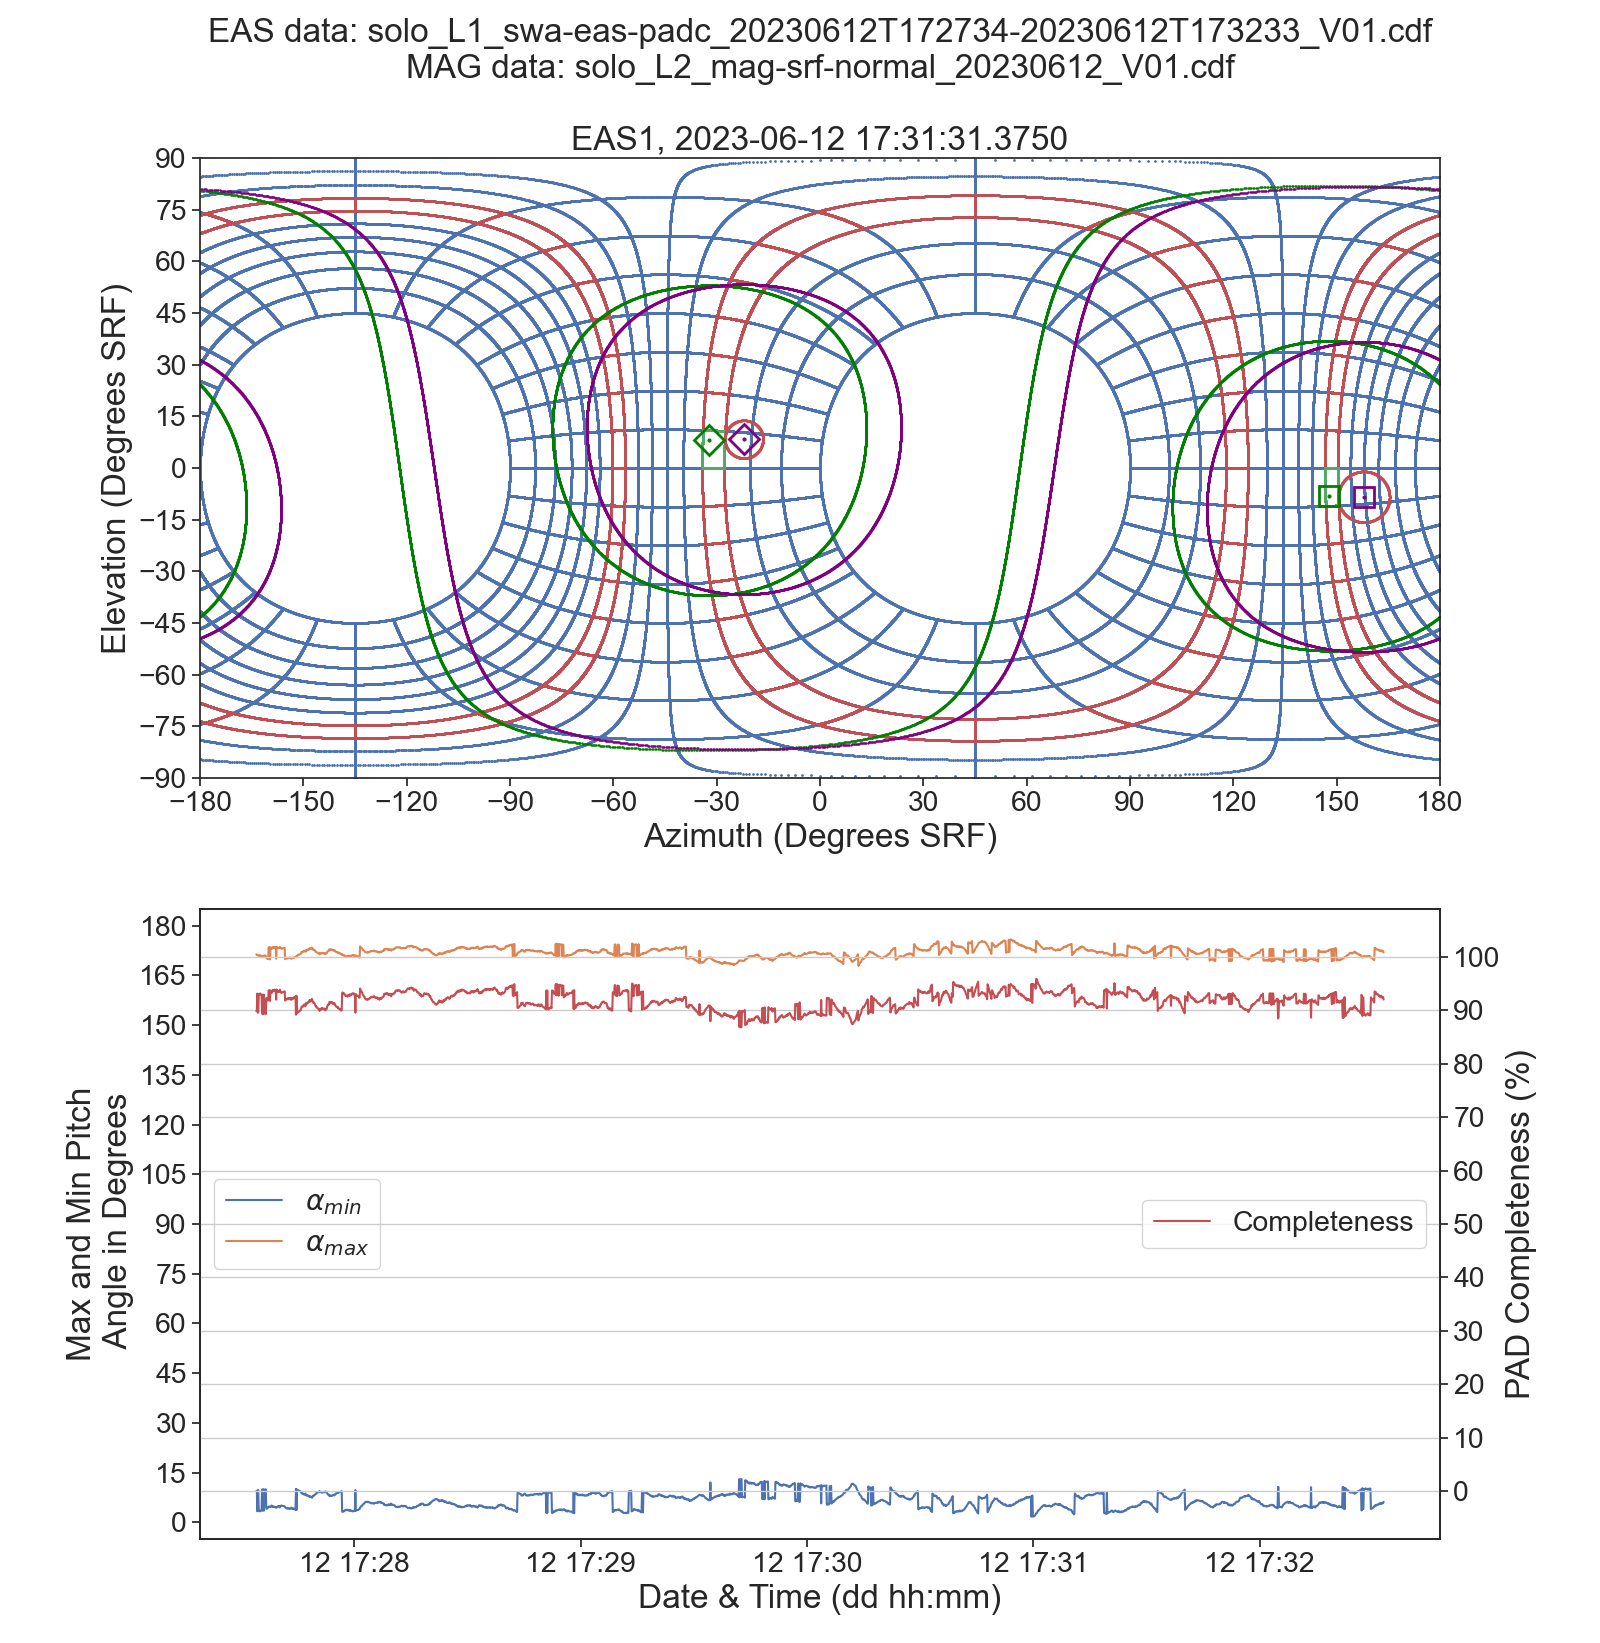
\includegraphics[width=1.2\linewidth]{figures/Verbose Example 12062023.png}
    \caption{Top panel: A plot of magnetic field vectors and calculated bin selection from 12th June 2023. Diamond and square markers represent parallel and anti-parallel magnetic field vectors respectively. Green represents \Beas\ and purple represents \Bmag. \(\alpha_{min}\) and \(\alpha_{max}\) are plotted as contours in red. Bottom panel: A plot of min and max pitch angles \(\alpha_{min}\) and \(\alpha_{max}\) and PAD completeness \textit{C} over the same period. \(\alpha_{min}\) and \(\alpha_{max}\) are plotted on the angular axis on the left, and \textit{C} is plotted on the percentage axis on the right.}
    \caption*{Image Source: Author's own work}
    \label{fig: full contours + selection + loss}
\end{figure}

The total angular loss in a Burst Mode PAD depends on the combined contributions of the parallel and anti-parallel losses \(\Delta_{\ppara}\) and \(\Delta_{\apara}\). Subtracting the total loss from the full \([0\degree-180\degree]\) range of an ideal PAD with lossless binning and steering gives the widest theoretical range of pitch angles that can be captured by that PAD. Taking the size of that range as a fraction of a full 180\degree\ yields the following metric of the PAD's completeness \textit{C}, where all angles are expressed in degrees:

\begin{equation} \label{eq: completeness}
    C=\frac{180\degree-\Delta_{\apara}-\Delta_{\ppara}}{180\degree}=\frac{\alpha_{max}-\alpha_{min}}{180\degree}
\end{equation}

\newpage
In summary, an algorithm for calculating the completeness of a Burst Mode PAD at a particular point in time \textit{t} can be described as follows:
\begin{enumerate} \label{alg: C algorithm}
    \item Acquire the upper and lower boundaries of the parallel and anti-parallel elevation bins selected by SWA-DPU at \textit{t}. In terms of the variables in SOAR EAS L1 \textit{.cdf} files, these boundaries can be calculated by summing the vectors from \q{SWA\_EAS\_ELEVATION} and \q{SWA\_EAS\_ELEVATION\_delta\_upper},  and from \q{SWA\_EAS\_ELEVATION} and \q{SWA\_EAS\_ELEVATION\_delta\_lower} at \textit{t} respectively.

    \item Acquire the EAS sensor head selected by SWA-DPU at \textit{t}. In terms of the variables in SOAR EAS L1 \textit{.cdf} files, these can be found under \q{SWA\_EAS\_EasUsed}.
    
    \item Identify the 8Hz MAG dataset containing the contemporaneous \Bmag\ vector at \textit{t}, and acquire the parallel and anti-parallel \Bmag\ vectors for that time. For simplicity, this dataset should be chosen such that the \Bmag\ vectors are already in cartesian SRF coordinates (see Section \ref{data}).

    \item Using the transformation matrices in the right column of Table \ref{tab: EASX to SRF}, transform the parallel and anti-parallel \Bmag\ vectors from cartesian SRF coordinates to the cartesian coordinates of the EAS sensor head selected at \textit{t} (\q{EASX}).

    \item Transform the parallel and anti-parallel \Bmag\ vectors from cartesian EASX coordinates to spherical EASX coordinates, and acquire their elevation angles in the range \([-90\degree,+90\degree]\)\footnote{Even though each EAS head can only sample the elevation range \([-45\degree,+45\degree]\), \Bmag\ vectors are not prevented from having an elevation outside of that range.}. 

    \item For each of the parallel and anti-parallel \Bmag\ vectors, check if their elevation angles are correctly binned by checking if they are between the upper and lower selected elevation bin boundaries. If either one is already correctly binned, then its associated loss is zero. 

    \item For each vector that is not already correctly binned, calculate the difference between its elevation and the elevation of the upper and lower selected elevation bin boundaries. The smallest of those two differences represents \(\Delta_{\ppara}\) for the parallel \Bmag\ vector or \(\Delta_{\apara}\) for the anti-parallel \Bmag\ vector.

    \item Use \(\Delta_{\ppara}\) and \(\Delta_{\apara}\) to calculate \textit{C} at \textit{t} according to Equation \ref{eq: completeness}.
\end{enumerate}
\\

\noindent This algorithm is relatively inexpensive to compute when compared to an alternative approach where EAS L1 data are completely re-binned into an accurate PAD and the missing pitch angle bins are counted manually. This is an algorithm that could be computed shortly after the receipt of EAS L1 data on the condition that contemporaneous MAG data are also downlinked and post-processed on the ground in a timely manner. Furthermore, the convenience of expressing PAD completeness as a single number, \textit{C}, may allow for faster determination of useful/unusable PADs for specific research purposes. For example, when investigating narrow, field-aligned electron strahl populations, high-\textit{C} may be a necessity to avoid missing all or most of the beams being studied. On the other hand, PADs with very low \textit{C} might be expected to have a limited range of pitch angle measurements, but multiple measurements of the same pitch few angles at varying gyrophase angles. Repeated measurements of the same pitch angle are redundant under the assumption of gyrotropy, but 8Hz measurements of gyrophase may provide a way to test that assumption using science data that are already available on SOAR, which \textit{C} could be used to identify\cite{owen2021}.
\\

While \textit{C} represents the theoretical maximum fraction of pitch angles available in a PAD, the effective range also depends on the choice of pitch angle binning. When EAS Burst Mode was introduced by Owen et al (2021), it was proposed that EAS VDFs could be resampled into eighteen 10\degree-wide pitch angle bins (this can be seen in the example in Figure \ref{fig: PAD example})\cite{owen2021}. If this number of bins is kept constant, then pitch angle loss would cause the bins at either end of the distribution either not to be \q{filled} or to be completely empty; their own form of incompleteness. Incomplete bins, if not completely discarded, should be analysed with caution as they may lead to misleading conclusions about the true electron PAD. Another approach is to vary the bin width, uniformly or non-uniformly, to maximise the actual range of pitch angles that can be analysed. In large datasets with varying completeness, the range of usable pitch angles may have to be sacrificed for the convenience of using standardised bin widths and bin numbers.
\\

So far, only the discrepancy between \(B_{EAS}\) and \(B_{MAG}\) has been examined for its effect on PAD completeness. However, the binning issue described in Section \ref{sim steering} should be expected to have its own effects on PAD completeness. Luckily, these effects are expected to be completely captured by the completeness algorithm. The binning issue concerns the discrepancy between \(B_{EAS}\) and its selected elevation bins, while the completeness algorithm concerns the discrepancy between \(B_{MAG}\) and the selected elevation bins. Whether or not these elevation bins were selected correctly for \(B_{EAS}\) only affects the completeness score indirectly depending on the agreement between \(B_{EAS}\) and \(B_{MAG}\). In fact, given sufficient disagreement between \(B_{EAS}\) and \(B_{MAG}\), the binning issue may lead \(B_{MAG}\) to be binned \textit{more accurately} than \(B_{EAS}\) (for example, if \(B_{EAS}\) lies outside the selected bin while \(B_{MAG}\), by chance, lies inside the selected bin).
\\

In Figure \ref{fig: full contours + selection + loss}, \(\alpha_{min}\) and \(\alpha_{max}\) have been calculated using binning according to the 17th July 2021 bin tables from SOAR (see Appendix \ref{appendixlabel1}). The binning issue described in Section \ref{sim steering} makes this calculation inaccurate. By extension, Figure \ref{fig: full contours + selection + loss} is also inaccurate. A more accurate figure can be generated by calculating \(\alpha_{min}\) and \(\alpha_{max}\) with the actual bins selected. The result of reproducing Figure \ref{fig: full contours + selection + loss} with this \q{corrected} approach is Figure \ref{fig: full contours + REAL selection + loss}. By comparing Figure \ref{fig: full contours + selection + loss} and Figure \ref{fig: full contours + REAL selection + loss}, it can be seen that \(\alpha_{min}\) is significantly higher in the latter plot (\(\sim15\degree\)) than in the former plot (\(\sim5\degree\)), meaning that \(\Delta_{\ppara}\) is larger as a consequence of the wrongly-selected elevation bin being farther from both \(B_{EAS, \ppara}\) and \(B_{MAG, \ppara}\). In contrast, it can also be seen that \(\alpha_{max}\) is somewhat higher in the latter plot (\(\sim175\degree\)) than in the former plot (\(\sim170\degree\)), meaning that \(\Delta_{\apara}\) is \textit{smaller} as a consequence of the wrongly-selected elevation bin being farther from \(B_{EAS, \apara}\) but closer to \(B_{MAG, \apara}\) by coincidence.
\\

\begin{figure}[h!]
    \centering
    \centerfloat
    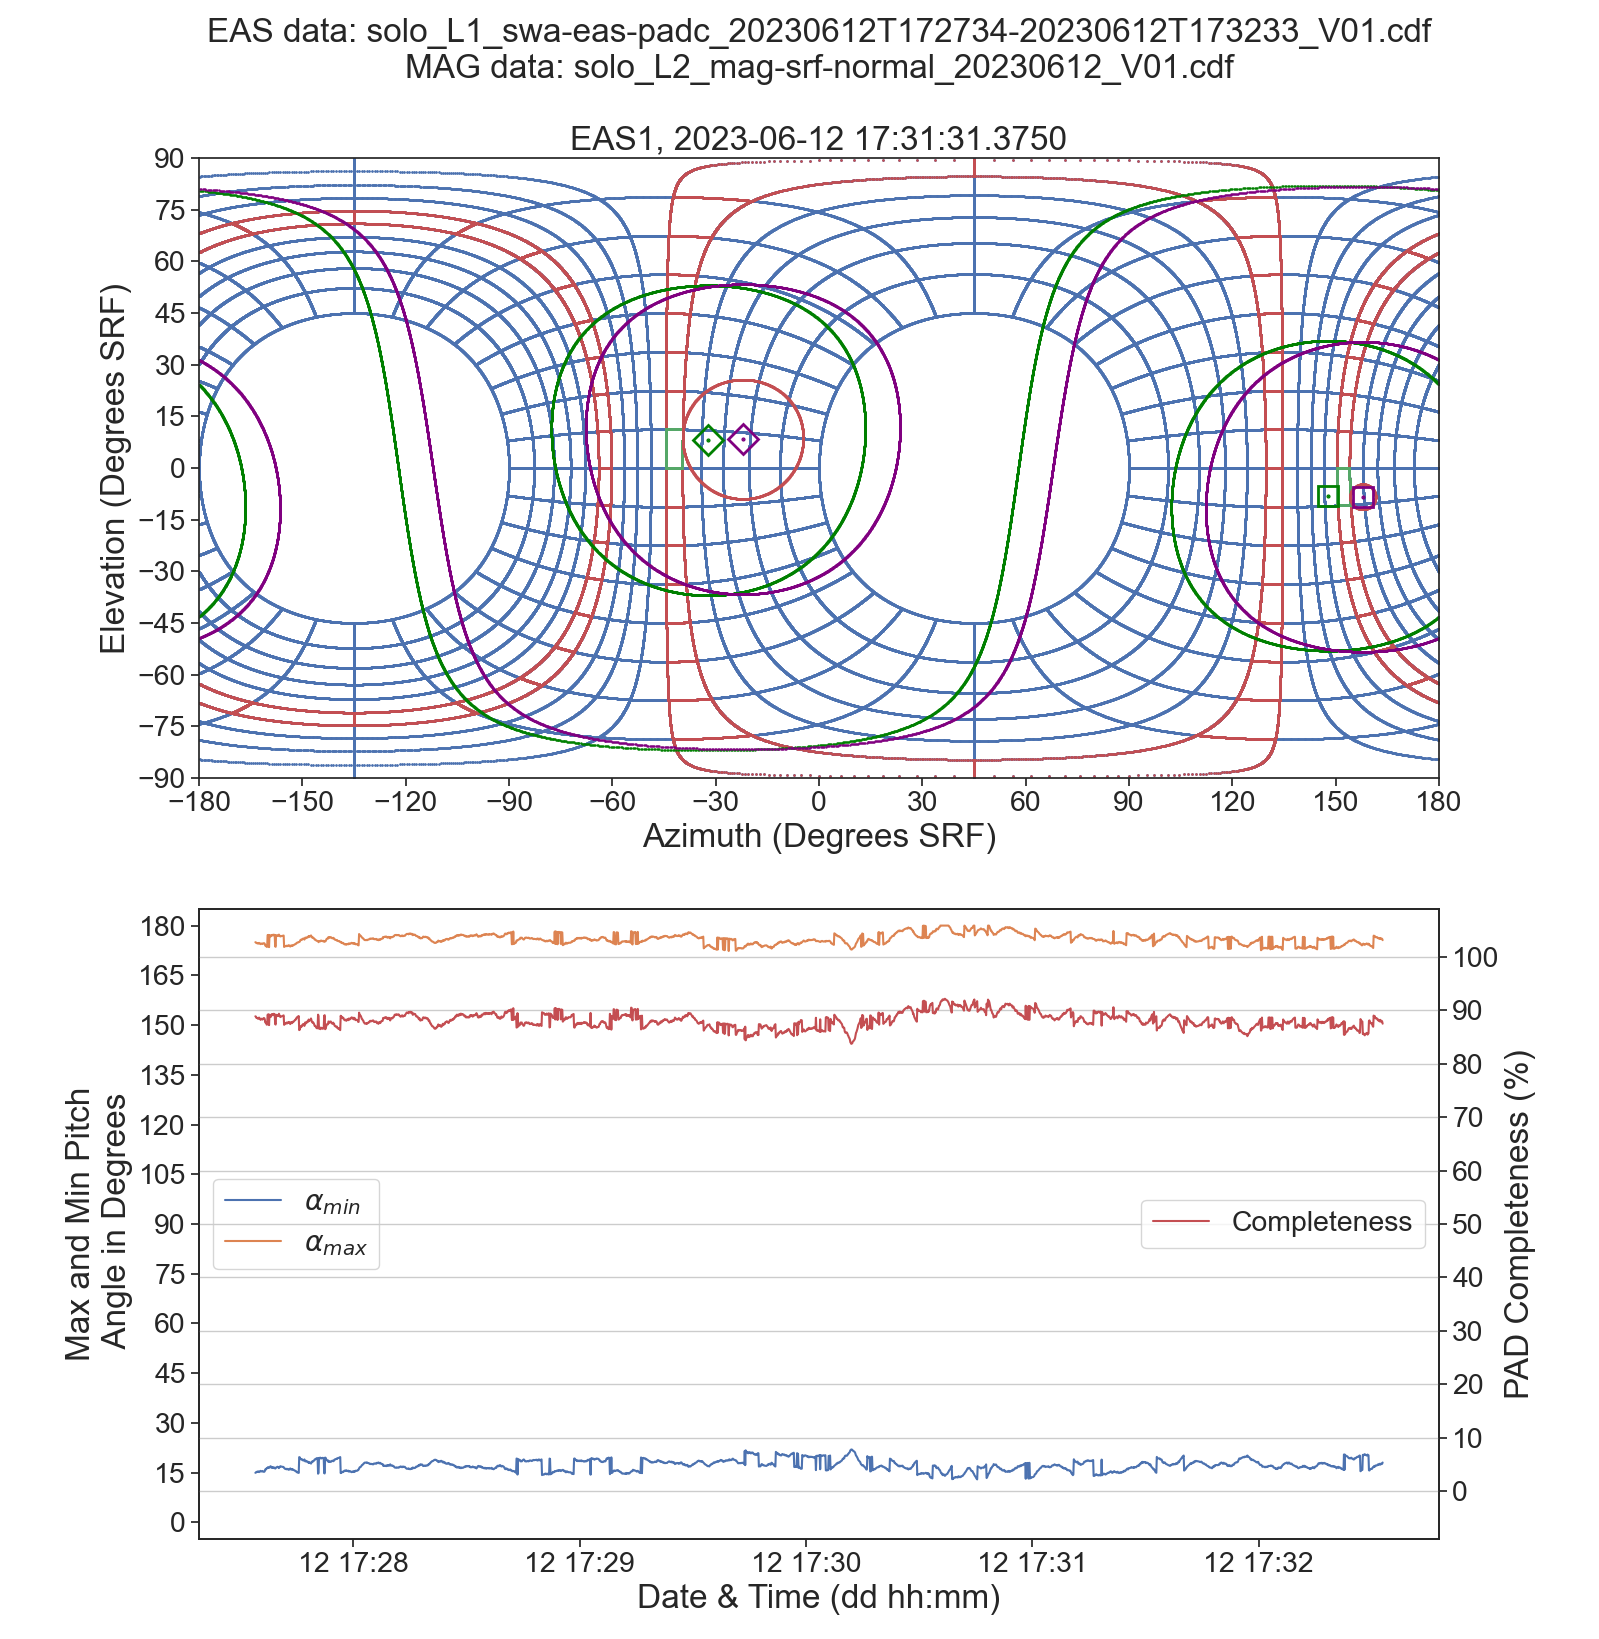
\includegraphics[width=1.2\linewidth]{figures/Verbose Example 12062023 Real.png}
    \caption{Top panel: A plot of magnetic field vectors and bin selection from 12th June 2023, where the binning issue is visible. Diamond and square markers represent parallel and anti-parallel magnetic field vectors respectively. Green represents \Beas\ and purple represents \Bmag. \(\alpha_{min}\) and \(\alpha_{max}\) are plotted as contours in red. Bottom panel: A plot of min and max pitch angles \(\alpha_{min}\) and \(\alpha_{max}\) and PAD completeness \textit{C} over the same period. \(\alpha_{min}\) and \(\alpha_{max}\) are plotted on the angular axis on the left, and \textit{C} is plotted on the percentage axis on the right.}
    \caption*{Image Source: Author's own work}
    \label{fig: full contours + REAL selection + loss}
\end{figure}

Equation \ref{eq: completeness} assumes the use of a basic VDF re-binning pipeline where pitch angles in the range \([0\degree,>90\degree]\) are re-binned from the parallel selected elevation bin and pitch angles in the range \([<90\degree,180\degree]\) are re-binned from the anti-parallel selected elevation bin. However, with sufficient disagreement between \(B_{EAS}\) and \(B_{MAG}\), it is theoretically possible for \(B_{MAG, \ppara}\) to be closer to either boundary of the \textit{anti}-parallel selected elevation bin than it is to the parallel selected elevation bin. Therefore, in that scenario, there may be a theoretical reduction in loss if the pitch angles in the range \([0\degree,>90\degree]\) were re-binned from the \textit{anti}-parallel selected elevation bin instead of the parallel selected elevation bin. This scenario is particularly likely if \(B_{EAS}\) is close to the selected EAS head's aperture center plane, because this should cause EAS to select parallel and anti-parallel elevation bins that are close to each other. An example of this phenomenon is found in Burst Mode data from 1st January 2023, and is shown in Figure \ref{fig: para antipara crossover} along with contours for \(\alpha_{min}\) and \(\alpha_{max}\) as calculated using Equations \ref{eq: alpha min} and \ref{eq: alpha max} respectively. In Figure \ref{fig: para antipara crossover}, the two selected elevation bins are adjacent to each other, and \(B_{MAG, \ppara}\) lies inside a different elevation bin than \(B_{EAS, \ppara}\). Although \(\alpha_{min}\) is still calculated and plotted under the assumption that it will be recovered from the parallel elevation bin, it is possible that \(\alpha_{min}\) (and therefore \(\Delta_{\ppara}\)) could be eliminated entirely if the anti-parallel elevation bin, in which \(B_{MAG, \ppara}\) lies, was used instead.
\\

This alternative approach would imply alternative calculations for the loss, yielding \(\Delta_{alt, \ppara}\) and \(\Delta_{alt, \apara}\), which are given by Equations \ref{eq: loss para _alt} and \ref{eq: loss anti _alt}.  These equations differ from Equations \ref{eq: parallel loss} and \ref{eq: antiparallel loss} in that \(\theta_{MAG, \ppara}\) and \(\theta_{MAG, \apara}\) are each compared to the elevations of \textit{all four} boundaries across both selected elevation bins instead of considering only the two boundaries of a single bin. In this case, the loss is given by the minimum angular distance of all four comparisons. As shown in Equations \ref{eq: loss para _alt} and \ref{eq: loss anti _alt}, this can be expressed succinctly by substituting \(\Delta_{\ppara}\) and \(\Delta_{\apara}\) for their equivalent expressions in Equations \ref{eq: parallel loss} and \ref{eq: antiparallel loss}.

\begin{equation} \label{eq: loss para _alt}
    \Delta_{alt, \ppara}=\min\{\Delta_{\ppara}, |\theta_{MAG, \ppara}-\theta_{upper, \apara}|, |\theta_{MAG, \ppara}-\theta_{lower, \apara}|\}
\end{equation}

\begin{equation} \label{eq: loss anti _alt}
    \Delta_{alt, \apara}=\min\{\Delta_{\apara}, |\theta_{MAG, \apara}-\theta_{upper, \ppara}|, |\theta_{MAG, \apara}-\theta_{lower, \ppara}|\}
\end{equation}

An equivalent completeness score \(C_{alt}\), is given by:

\begin{equation} \label{eq: C_alt}
    C_{alt}=\frac{180\degree-\Delta_{alt, \apara}-\Delta_{alt, \ppara}}{180\degree}
\end{equation}

\(C_{alt}\) can be incorporated into the algorithm for calculating \(C\) presented on page \pageref{alg: C algorithm} by changing steps 6 and 7 to require both the parallel and anti-parallel selected bins to be checked and compared against the \Bmag\ vector, and by changing step 8 to use Equation \ref{eq: C_alt}.
\\

\begin{figure}[h!]
    \centering
    \centerfloat
    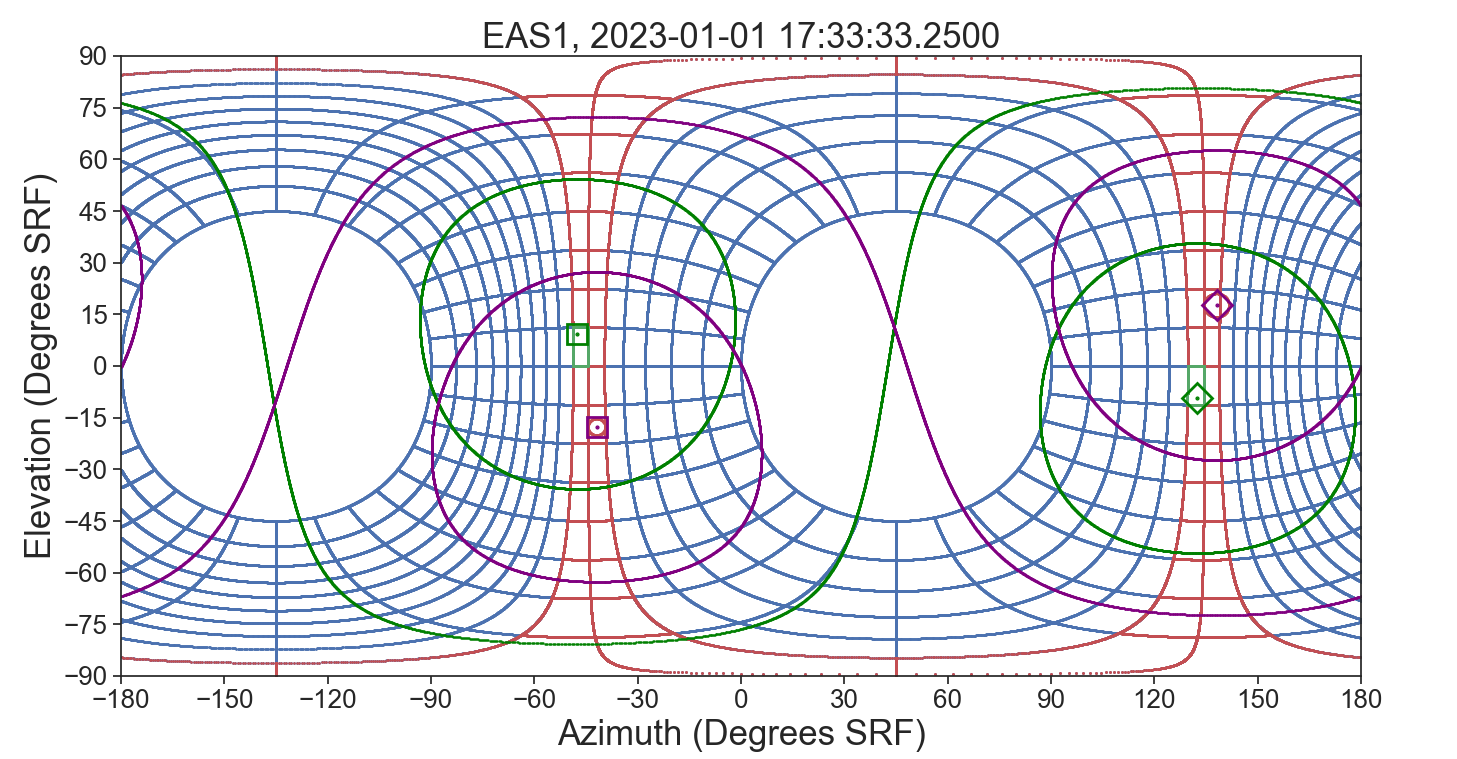
\includegraphics[width=1.1\linewidth]{figures/Crossover Example.png}
    \caption{A plot of magnetic field vectors and calculated bin selection from 1st January 2023, where the parallel and anti-parallel elevation bins are adjacent to each other. Diamond and square markers represent parallel and anti-parallel magnetic field vectors respectively. Green represents \Beas\ and purple represents \Bmag. \(\alpha_{min}\) and \(\alpha_{max}\) are plotted as (barely visible) contours in red.}
    \caption*{Image Source: Author's own work}
    \label{fig: para antipara crossover}
\end{figure}


\noindent \(C\), \(C_{alt}\) and the algorithms used to calculate them represent two relatively inexpensive approaches to determining the completeness of any given Burst Mode PAD based only on data for the contemporaneous MAG vector used (\Bmag) and the EAS elevation bins selected. In particular, \(C\) and its associated losses and min/max pitch angles have been calculated and presented for various instances of randomly selected sample data in this report, but future work could investigate the long-term variation of \textit{C}, collating months or years of EAS Burst Mode data available from SOAR. This may reveal a relationship between completeness and the time elapsed since the last routine calibration update to correct MAG offset drift, or a relationship between completeness and the rate of change of the magnetic field, potentially driven by magnetic turbulence in the solar wind\cite{smith2021}. 

\newpage
\section{S20 Link Latency} \label{S20 Link Latency}

To test the S20 latency algorithm described in Section \ref{S20 method} using real magnetic field data, a sample of \Bmag\ data from 30th May 2023 was given a large, artificial time offset of 50s and cross-correlated with itself, yielding two versions of it to represent an equivalent of \(f(t)\) and \(g(t)\) as previously described. The result for the \Bmag\ elevation in EAS1 coordinates is presented in Figure \ref{fig: arti 50s}. Only a single axis is considered here to avoid having to combine different measurements of the time delay from different axes, as described in detail in the author's previous work\cite{dickson2024}. The precision here is surprisingly high, yielding \(\tau_r=49.9\textrm{s}\pm1.8\)s, and the error bar associated with this uncertainty is barely visible on the lower panel of Figure \ref{fig: arti 50s}. The algorithm was then applied again, with a shorter time delay of 5s, yielding Figure \ref{fig: arti 5s}. Surprisingly again, the precision in this case was also high, yielding \(\tau_r=4.90\textrm{s}\pm0.2\)s. If this trend in increasing precision continues, then the S20 latency algorithm may be able to accurately characterise real differences between \Bmag\ and \Beas\ data more effectively than the author's previous attempts\cite{dickson2024}. This is an exciting subject that warrants future investigation.

\begin{figure}[h!]
    \centering
    \centerfloat
    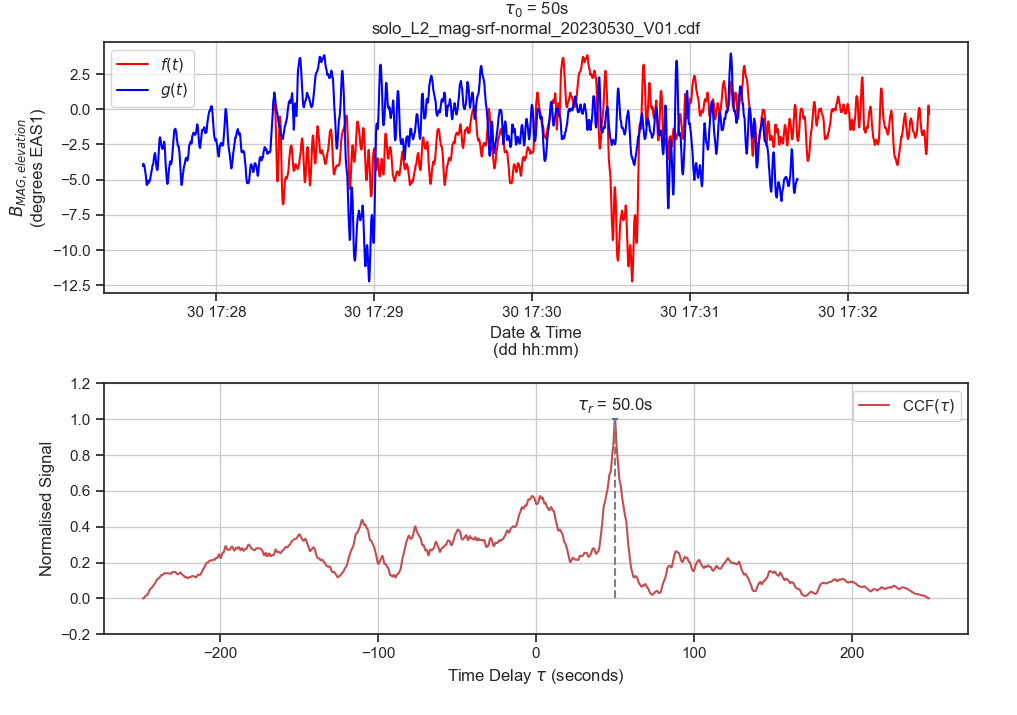
\includegraphics[width=1.3\linewidth]{figures/artificial delay 50s.png}
    \caption{Top panel: Two \q{identical} plots of \Beas\ elevation in EAS1 coordinates with an artificial, 50s time delay between them. Bottom panel: The result of the CCF algorithm applied to the top panel, where the uncertainty in \(\tau_r\) is indicated by the small, horizontal, blue bar.}
    \caption*{Image Source: Author's own work}
    \label{fig: arti 50s}
\end{figure}

\begin{figure}[h!]
    \centering
    \centerfloat
    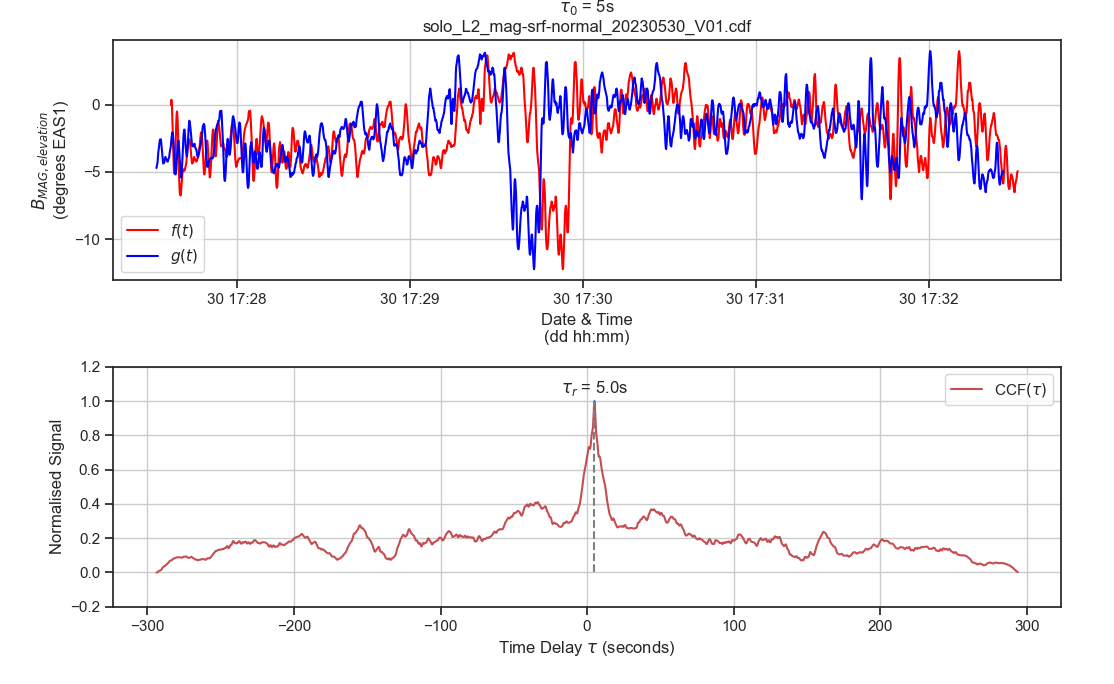
\includegraphics[width=1.35\linewidth]{figures/artificial delay 5s.png}
    \caption{Top panel: Two \q{identical} plots of \Beas\ elevation in EAS1 coordinates with an artificial, 5s time delay between them. Bottom panel: The result of the CCF algorithm applied to the top panel.}
    \caption*{Image Source: Author's own work}
    \label{fig: arti 5s}
\end{figure}